\documentclass[a4paper,14pt]{extarticle}

\usepackage[utf8x]{inputenc}
\usepackage[T1,T2A]{fontenc}
\usepackage[russian]{babel}
\usepackage{hyperref}
\usepackage{indentfirst}
\usepackage{here}
\usepackage{array}
\usepackage{graphicx}
\usepackage{caption}
\usepackage{subcaption}
\usepackage{chngcntr}
\usepackage{amsmath}
\usepackage{pgfplots}
\usepackage{pgfplotstable}
\usepackage[left=2cm,right=2cm,top=2cm,bottom=2cm,bindingoffset=0cm]{geometry}

\counterwithin{figure}{section}
\counterwithin{equation}{section}
\counterwithin{table}{section}
\newcommand{\sign}[1][5cm]{\makebox[#1]{\hrulefill}} % Поля подписи и даты
\graphicspath{{pics/}} % Путь до папки с картинками

\begin{document}

\begin{titlepage}
	\begin{center}
		\textbf{Санкт-Петербургский Политехнический Университет Петра Великого}\\[0.3cm]
		\small Институт компьютерных наук и технологий \\[0.3cm]
		\small Кафедра компьютерных систем и программных технологий\\[4cm]
		
		\textbf{ОТЧЕТ}\\ \textbf{о лабораторной работе}\\[0.5cm]
		\textbf{Исследование частотных характеристик пассивных RC-цепей}\\[0.1cm]
		\textbf{Электротехника и Электроника}\\[10.5cm]
	\end{center}
	
	\begin{flushright}
		\begin{minipage}{0.60\textwidth}
			\begin{flushleft}
				\small \textbf{Работу выполнили студенты}\\[3mm]
				\small группа 23501/4 \hspace*{17mm} Дьячков В.В.\\[3mm]
				\small группа 23501/4 \hspace*{17mm} Ламтев А.Ю.\\[5mm]
				
				\small \textbf{Преподаватель}\\[5mm]
			 	\small \sign[3.5cm] \hspace*{8mm} к.т.н., доц. Кочетков Ю.Д.\\[0.5cm]
			\end{flushleft}
		\end{minipage}
	\end{flushright}
	
	\vfill
	
	\begin{center}
		\small Санкт-Петербург\\
		\small \the\year
	\end{center}
\end{titlepage}

\section{Цель работы}

Исследовать частотные свойства простейших пассивных RC­-цепей и познакомиться с правилами построения частотных характеристик.

\section{Чертеж схемы исследуемого устройства}

\begin{figure}[H]
\begin{center}
	\begin{subfigure}[b]{0.3\textwidth}
		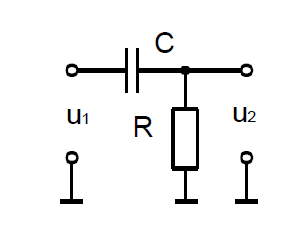
\includegraphics[scale=0.4]{diff}
		\caption{Дифференцирующая\\ цепь}
	\end{subfigure}
	\begin{subfigure}[b]{0.3\textwidth}
		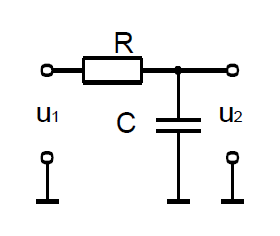
\includegraphics[scale=0.4]{int}
		\caption{Интегрирующая\\ цепь}
	\end{subfigure}
	\begin{subfigure}[b]{0.3\textwidth}
		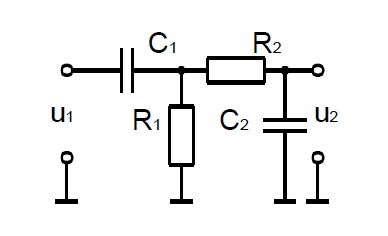
\includegraphics[scale=0.4]{diff-int}
		\captionsetup{justification=centering}
		\caption{Дифференцирующая и интегрирующая цепь}
	\end{subfigure}
	\caption{}
\end{center}
\end{figure}

\section{Исходные данные}

\begin{table}[H]
\begin{center}
	\caption{Исходные данные}
	\renewcommand\arraystretch{1.3}
	\renewcommand\tabcolsep{50pt}
	\begin{tabular}{|c|c|}
		\hline
		$R$, кОм & $C$, нФ\\
		\hline
		15 & 5\\
		\hline	
	\end{tabular}
\end{center}
\end{table}

\section{Теоретические зависимости}

Частота перегиба расcчитывается следующим образом:
\begin{equation}
	\omega_0 = \frac{1}{RC} = \frac{1}{15 \cdot 10^3 \cdot 5 \cdot 10^{-9}} \approx 1.334 \cdot 10^4 \hspace*{2mm}
\end{equation}

Рассчитаем $f_0$: 
\begin{equation}
	f_0 = \frac{\omega_0}{2 \pi} = \frac{1.34}{2\cdot1.341} \approx 2122.065 (\text{Гц})
\end{equation}

Теоретическая ЛАЧХ для дифференцирующей RC-цепи имеет вид:
\begin{equation}\label{eq:l_diff}
	L_u^1(\omega) = 20\lg \omega RC - 10\lg (1+(\omega RC)^2),
\end{equation}

Теоретическая ЛАЧХ для интегрирующей RC-цепи имеет вид:
\begin{equation}\label{eq:l_int}
	L_u^2(\omega) = -10\lg (1+(\omega RC)^2),
\end{equation}

Теоретическая ЛАЧХ для дифференцирующей и интегрирующей RC-цепи имеет вид:
\begin{equation}\label{eq:l_diff_int}
	L_u^3(\omega) = 20\lg \omega RC - 10\lg (1+7(\omega RC)^2 + (\omega RC)^4).
\end{equation}

При помощи формул \ref{eq:l_diff}, \ref{eq:l_int} и \ref{eq:l_diff_int} была составлена таблица \ref{tab:bode}.

\begin{table}[H]
\begin{center}
	\caption{Значения для построения теоретических ЛАЧХ}\label{tab:bode}
	\renewcommand\arraystretch{1.3}
	\renewcommand\tabcolsep{17pt}
	\pgfplotstabletypeset[col sep=comma,
	    columns={f,w,diff,int,diff-int},
	    column type/.add={|c|}{},
	    columns/f/.style={fixed, column name={$f$, Гц}},
	    columns/w/.style={fixed, precision=3, zerofill, column name={$\omega = 2 \pi f$}},
	    columns/diff/.style={fixed, precision=3, zerofill, column name={$L_u^1$, дБ}},
	    columns/int/.style={fixed, precision=3, zerofill, column name={$L_u^2$, дБ}},
	    columns/diff-int/.style={fixed, precision=3, zerofill, column name={$L_u^3$, дБ}},
	    every nth row={1}{before row=\hline},
	    every head row/.style = {before row=\hline, after row=\hline},
	    every last row/.style = {after row=\hline}
	   ]{data/bode.csv}
\end{center}
\end{table}

\newpage

\section{Экспериментально снятые зависимости}

В таблицах \ref{tab:diff}, \ref{tab:int} и \ref{tab:diff-int} приведены значения входного напряжения, выходного напряжения, коэффициента передачи и коэффициента передачи, выраженного в децибелах, дифференцирующей RC-цепи, интегрирующей RC-цепи и дифференцирующе-интегрирующей RC-цепи, представляющей собой последовательное соединение дифференцирующей и интегрирующей RC-цепей.

\begin{table}[H]
\begin{center}
	\caption{ЛАЧХ дифференциующей RC-цепи}\label{tab:diff}
	\renewcommand\arraystretch{1.3}
	\renewcommand\tabcolsep{20pt}
	\pgfplotstabletypeset[col sep=comma,
	    columns={f,u_in,u_out,k,lg_k},
	    column type/.add={|c|}{},
	    columns/f/.style={fixed, column name={$f$, Гц}},
	    columns/u_in/.style={fixed, precision=2, zerofill, column name={$U_\text{вх}$, В}},
	    columns/u_out/.style={fixed, precision=3, zerofill, column name={$U_\text{вых}$, В}},
	    columns/k/.style={fixed, precision=3, zerofill, column name={$K$, В}},
	    columns/lg_k/.style={fixed, precision=3, zerofill, column name={$20 \cdot \lg K$, дБ}},
	    every nth row={1}{before row=\hline},
	    every head row/.style = {before row=\hline, after row=\hline},
	    every last row/.style = {after row=\hline}
	   ]{data/diff.csv}
\end{center}
\end{table}

\begin{table}[H]
\begin{center}
	\caption{ЛАЧХ интегрирующей RC-цепи}\label{tab:int}
	\renewcommand\arraystretch{1.3}
	\renewcommand\tabcolsep{20pt}
	\pgfplotstabletypeset[col sep=comma,
	    columns={f,u_in,u_out,k,lg_k},
	    column type/.add={|c|}{},
	    columns/f/.style={fixed, column name={$f$, Гц}},
	    columns/u_in/.style={fixed, precision=2, zerofill, column name={$U_\text{вх}$, В}},
	    columns/u_out/.style={fixed, precision=3, zerofill, column name={$U_\text{вых}$, В}},
	    columns/k/.style={fixed, precision=3, zerofill, column name={$K$, В}},
	    columns/lg_k/.style={fixed, precision=3, zerofill, column name={$20 \cdot \lg K$, дБ}},
	    every nth row={1}{before row=\hline},
	    every head row/.style = {before row=\hline, after row=\hline},
	    every last row/.style = {after row=\hline}
	   ]{data/int.csv}
\end{center}
\end{table}

\begin{table}[H]
\begin{center}
	\caption{ЛАЧХ дифференцирующе-интегрирующей RC-цепи}\label{tab:diff-int}
	\renewcommand\arraystretch{1.3}
	\renewcommand\tabcolsep{20pt}
	\pgfplotstabletypeset[col sep=comma,
	    columns={f,u_in,u_out,k,lg_k},
	    column type/.add={|c|}{},
	    columns/f/.style={fixed, column name={$f$, Гц}},
	    columns/u_in/.style={fixed, precision=2, zerofill, column name={$U_\text{вх}$, В}},
	    columns/u_out/.style={fixed, precision=3, zerofill, column name={$U_\text{вых}$, В}},
	    columns/k/.style={fixed, precision=3, zerofill, column name={$K$, В}},
	    columns/lg_k/.style={fixed, precision=3, zerofill, column name={$20 \cdot \lg K$, дБ}},
	    every nth row={1}{before row=\hline},
	    every head row/.style = {before row=\hline, after row=\hline},
	    every last row/.style = {after row=\hline}
	   ]{data/diff-int.csv}
\end{center}
\end{table}


\newpage

\section{Построение эксперментальных ЛАЧХ}

На рисунках \ref{fig:diff}, \ref{fig:int} и \ref{fig:diff-int} приведены теоритические ЛАЧХ, экспериментальные ЛАЧХ и аппроксимирующие прямые для всех цепей.

\begin{figure}[H]
\begin{center}
	\begin{tikzpicture}
		\begin{axis}[
			height=0.4\textheight,
			width=0.9\textwidth,
			legend pos=south east,
			xlabel={$f$, Гц},
			ylabel={$L_u^1$, дБ},
			xlabel near ticks,
			ylabel near ticks,
			ymin=-40,
			xmode=log,
			log basis x=2,
			xtick={0, 32, 128, 512, 2048, 8192, 32768, 131072},
			xtick pos=right,
			grid=major
		]
		\addplot table [x=f, y=diff, col sep=comma] {data/bode.csv};
		\addplot table [x=f, y=lg_k, col sep=comma] {data/diff.csv};
		\addplot +[mark=none, dashed, black, samples=2] coordinates {(2048,0) (200000,0)};
		\addplot +[mark=none, dashed, black, domain=32:2048] {-(log2(x)*(-6)+66.3)};
		\legend{Teор. ЛАЧХ, Эксп. ЛАЧХ, Аппроксимация}
		\end{axis}
	\end{tikzpicture}
	\captionsetup{justification=centering,margin=2cm}
	\caption{Теоретическая и экспериментальная ЛАЧХ дифференцирующей RC-цепи}\label{fig:diff}
\end{center}
\end{figure}

\renewcommand\belowcaptionskip{-40pt}

\begin{figure}[H]
\begin{center}
	\begin{tikzpicture}
		\begin{axis}[
			height=0.4\textheight,
			width=0.9\textwidth,
			legend pos=south west,
			xlabel={$f$, Гц},
			ylabel={$L_u^2$, дБ},
			xlabel near ticks,
			ylabel near ticks,
			ymin=-40,
			xmode=log,
			log basis x=2,
			xtick={0, 32, 128, 512, 2048, 8192, 32768, 131072},
			xtick pos=right,
			grid=major
		]
		\addplot table [x=f, y=int, col sep=comma] {data/bode.csv};
		\addplot table [x=f, y=lg_k, col sep=comma] {data/int.csv};
		\addplot +[mark=none, dashed, black, samples=2] coordinates {(32,0) (2048,0)};
		\addplot +[mark=none, dashed, black, domain=2048:200000] {log2(x)*(-6)+66.3};
		\legend{Teор. ЛАЧХ, Эксп. ЛАЧХ, Аппроксимация}
		\end{axis}
	\end{tikzpicture}
	\captionsetup{justification=centering,margin=2cm}
	\caption{Теоретическая и экспериментальная ЛАЧХ интегрирующей RC-цепи}\label{fig:int}
\end{center}
\end{figure}

\renewcommand\belowcaptionskip{0pt}

\begin{figure}[H]
\begin{center}
	\begin{tikzpicture}
		\begin{axis}[
			height=0.4\textheight,
			width=0.9\textwidth,
			legend pos=north east,
			xlabel={$f$, Гц},
			ylabel={$L_u^3$, дБ},
			xlabel near ticks,
			ylabel near ticks,
			xmode=log,
			log basis x=2,
			xtick={0, 32, 128, 512, 2048, 8192, 32768, 131072},
			xtick pos=right,
			grid=major
		]
		\addplot table [x=f, y=diff-int, col sep=comma] {data/bode.csv};
		\addplot table [x=f, y=lg_k, col sep=comma] {data/diff-int.csv};
		\addplot +[mark=none, dashed, black, domain=2048:200000] {log2(x)*(-6)+66.3};
		\addplot +[mark=none, dashed, black, domain=32:2048] {-(log2(x)*(-6)+66.3)};
		\legend{Teор. ЛАЧХ, Эксп. ЛАЧХ, Аппроксимация}
		\end{axis}
	\end{tikzpicture}
	\captionsetup{justification=centering,margin=2cm}
	\caption{Теоретическая и экспериментальная ЛАЧХ дифференцирующе-интегрирующей RC-цепи}\label{fig:diff-int}
\end{center}
\end{figure}

\section{Погрешности}

\subsection{Предельно допустимые погрешности}

\begin{center}
$\delta R = 0.1 = 10\%$\\
$\delta C = 0.1 = 10\%$\\
\end{center}

\subsubsection{Дифференцирующей и интегрирующей цепей}

Дифференцирующая и интегрирующая цепи включают в себя по одному резистору и по одному конденсатору, поэтому предельно допустимая относительная погрешность частоты перегиба вычисляется следующим образом:
\[
\delta f_0 = \sqrt{(\delta R)^2 + (\delta C)^2} = \sqrt{0.1^2 + 0.1^2} = \sqrt{0.02} = 0.141 = 14.1 \%
\]

\subsubsection{Дифференцирующе-интегрирующей цепи}

Дифференцирующе-интегрирующая цепь содержит два резистора и два конденсатора, поэтому предельно допустимая относительная погрешность частоты перегиба вычисляется по формуле:
\[
\delta f_0 = \sqrt{2 \cdot ((\delta R)^2 + (\delta C)^2)} = \sqrt{2 \cdot (0.1^2 + 0.1^2)} = \sqrt{0.04} = 0.2 = 20 \%
\]

\subsection{Расчет значения $f$}

Необходимо рассчитать значение частоты $f$, при которой коэффициент передачи равен $-3$~дБ для дифференцирующей и интегрирующей цепей и $-9$~дБ для последовательного соединения дифференцирующей и интегрирующей цепей. Построим интерполяционный полином Лагранжа по 3-м точкам (2-й степени), наиболее близким к теоретической $f_0 = 2122.065$~Гц: $1024$~Гц, $2048$~Гц и $4096$~Гц.

\subsubsection{Для дифференцирующей RC-цепи}

Для дифференцирующей RC-цепи интерполирующий полином имеет вид:
\[
Q_2(x) = (-9.474 \cdot 10^{-7})x^2 + (6.81 \cdot 10^{-3})x - 13.393
\]

Искомая частота равна f, такому, что $Q_2(f) = -3$:
\[
(-9.474 \cdot 10^{-7})f^2 + (6.81 \cdot 10^{-3})f -13.393 = -3 \Rightarrow f = 2197.92 \text{ Гц}
\]

Для полученного значения $f = 2197.92$ Гц рассчитаем погрешность:
\[
\delta f = \frac{|f_0 - f|}{f_0} = \frac{|2122.065 - 2197.92|}{2122.065} = 3.57 \% < \delta f_0 = 14.1\%
\]

\subsubsection{Для интегрирующей RC-цепи}

Для интергрирующей RC-цепи интерполирующий полином представим в виде:
\[
Q_2(x) = (1.303 \cdot 10^{-8})x^2 - (2.013 \cdot 10^{-3})x + 0.744
\]

Искомая частота равна такому $f$, что $Q_2(f) = -3$:
\[
(1.303 \cdot 10^{-8})f^2 - (2.013 \cdot 10^{-3})f + 0.744 = -3 \Rightarrow f = 1882.39 \text{ Гц}
\]

Для полученного значения $f = 1882.39$ Гц рассчитаем погрешность:
\[
\delta f = \frac{|f_0 - f|}{f_0} = \frac{|2122.065 - 1882.39|}{2122.065} = 11.3 \% < \delta f_0 = 14.1\%
\]

\subsubsection{Дифференцирующе-интегрирующая цепь}

Интерполяционный полином дифференцирующе-интегрирующей RC-цепи имеет вид:\\
\[
Q_2(x) = (-4.242 \cdot 10^{-7})x^2 + (2.186 \cdot 10^{-3})x - 12.667
\]

Значение частоты перегиба - это то значение x, при котором 1-ая производная полинома обращается в 0:
\[
\frac{d}{dx} (Q_2(x))\Big|_{x=f} = 2 \cdot (-4.242 \cdot 10^{-7})f + (2.186 \cdot 10^{-3}) = 0 \Rightarrow f = 2576.62 (\text{Гц})
\]

Для полученного значения $f = 2576.62$ Гц рассчитаем погрешность:
\[
\delta f = \frac{|f_0 - f|}{f_0} = \frac{|2122.065 - 2576.62|}{2122.065} \approx 20 \% \leq \delta f_0 = 20\%
\]
  
\section{Выводы}

Вычисленные значения частоты перегиба для дифференцирующей, интегрирующей и дифференцирующе-интегрирующей RC-цепей имеют приведенную погрешность, которая не превосходит допустимую. 

Таким образом, формулы для вычисления теоретической ЛАЧХ \ref{eq:l_diff}, \ref{eq:l_int} и \ref{eq:l_diff_int} являются верными.

\end{document}
